\section{Light Sources}

\begin{frame}{Light in Nature}
  \begin{columns}
    \begin{column}{0.3\textwidth}
      \begin{tikzpicture}[scale=0.8]
        \node[circle, fill=LightColor, minimum size=1.5cm] (sun) at (2,4) {\Large\faIcon{sun}};
        \node[above] at (2,6) {\small \textcolor{LightColor}{Electromagnetic Radiation}};

        \foreach \angle in {0,30,60,90,120,150,180,210,240,270,300,330} {
          \draw[lightray, opacity=0.6] (sun) -- +(\angle:2);
        }

        \draw[ObjectColor, very thick] (0,0) -- (4,0);
        \node[below] at (2,-0.3) {\objectcolor{Surface}};

        \draw[reflectray] (1.5,0) -- (1,1.5);
        \draw[reflectray] (2.5,0) -- (2,1.5);
        \node[right] at (2.5,0.7) {\footnotesize Reflected};

        \node[red, below] at (2,-0.8) {\footnotesize Absorbed → Heat};
      \end{tikzpicture}
    \end{column}
    \pause
    \begin{column}{0.6\textwidth}
      \begin{conceptbox}{Physical Properties}
        \textbf{Light is electromagnetic radiation:}
        \begin{itemize}
            \footnotesize
          \item Wavelength determines color
          \item Intensity determines brightness
          \item Travels at speed of light ($c$)
          \item Behaves as waves and particles
        \end{itemize}

        \vspace{0.3cm}
        \textbf{Surface interactions:}
        \begin{itemize}
            \footnotesize
          \item \textbf{Reflection} (bounces off)
          \item Absorption (converts to heat)
          \item Transmission (passes through)
        \end{itemize}
      \end{conceptbox}
    \end{column}
  \end{columns}
\end{frame}

\subsection{Point Light}

\begin{frame}{Point Light Sources - Introduction}
  \begin{columns}
    \begin{column}{0.6\textwidth}
      \begin{raybox}{Point Light Characteristics}
        \small
        Light emanating from a single point in all directions

        \only<2->{
          \vspace{0.3cm}
          \textbf{Real-world examples:}
          \begin{itemize}
            \item Light bulbs, LEDs
            \item Candles
          \end{itemize}
        }
      \end{raybox}
    \end{column}
    \begin{column}{0.4\textwidth}
      \begin{tikzpicture}[scale=0.75]
        % Point light source
        \node[circle, fill=LightColor, minimum size=0.8cm] (light) at (2,2) {\faIcon{lightbulb}};
        \node[above] at (2,3.5) {\small \textcolor{LightColor}{Point Light}};

        % Omnidirectional rays
        \foreach \angle in {0,30,60,90,120,150,180,210,240,270,300,330} {
          \draw[lightray] (light) -- +(\angle:1.5);
        }

        % Objects at different distances
        \node[sphere, minimum size=0.8cm, fill=ObjectColor!20] (obj1) at (0,2) {};
        \node[sphere, minimum size=0.8cm, fill=ObjectColor!50] (obj2) at (5,2) {};

        % Distance labels
        \draw[<->, thin] (light) -- (obj1) node[midway, above] {\footnotesize $d_1$};
        \draw[<->, thin] (light) -- (obj2) node[midway, above] {\footnotesize $d_2$};

        % Intensity indication
        \node[below] at (0,1.2) {\footnotesize Brighter};
        \node[below] at (5,1.2) {\footnotesize Dimmer};
      \end{tikzpicture}
    \end{column}
  \end{columns}
  \only<3->{
    \vspace{0.1cm}
    \begin{center}
      \begin{figure}
        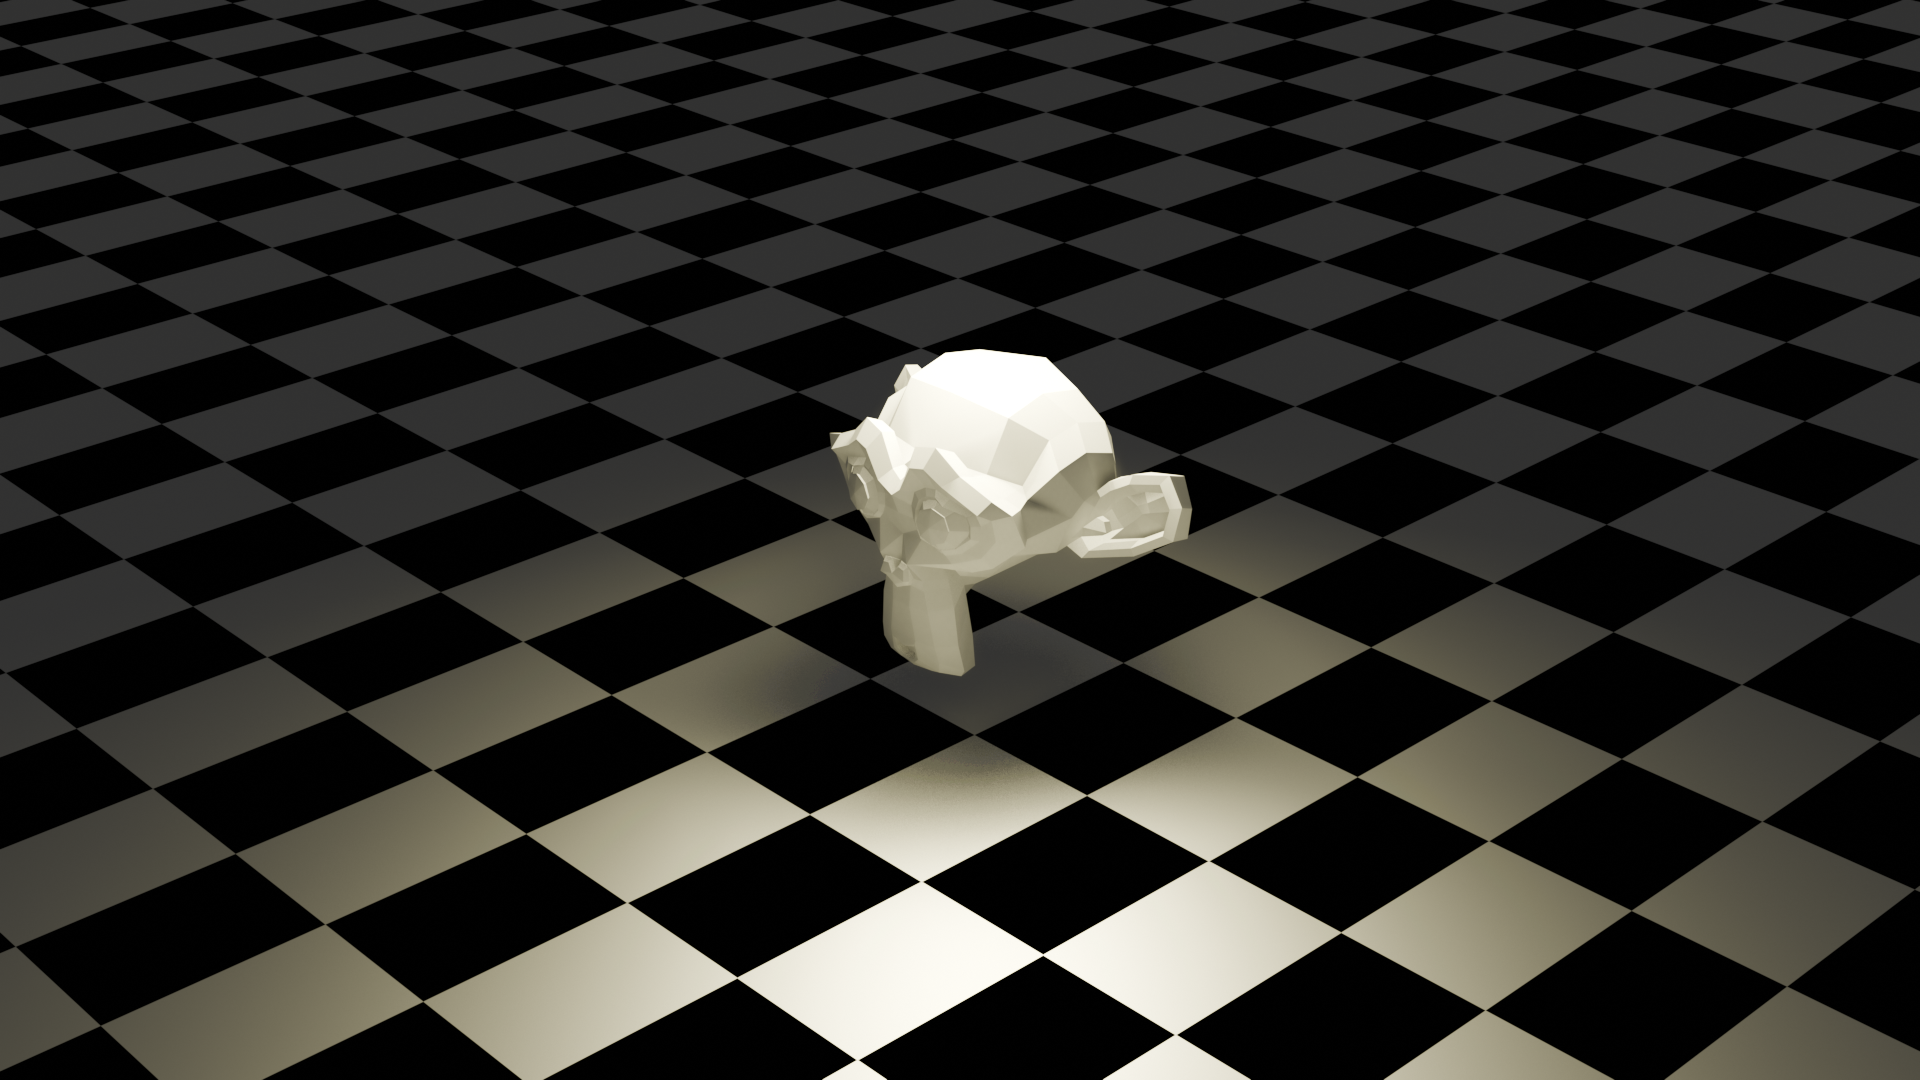
\includegraphics[width=0.5\linewidth]{images/point.png}
        \caption{Point Light ft. Suzanne the monkey}
      \end{figure}
    \end{center}
  }
\end{frame}

\begin{frame}{Point Light Mathematics}
  \begin{columns}
    \begin{column}{0.6\textwidth}
      \begin{mathbox}{Point Light Parameters}
        \textbf{Position:} $\mathbf{P}_{\text{light}} = (x_l, y_l, z_l)$

        \textbf{Intensity:} $I_{\text{light}}$ (brightness)

        \textbf{Color:} $\mathbf{C}_{\text{light}} = (r, g, b)$

        \vspace{0.3cm}
        \pause
        \textbf{Light direction to surface point:}
        \begin{align*}
          \mathbf{L} &= \mathbf{P}_{\text{light}} - \mathbf{P}_{\text{surface}} \\
          \hat{\mathbf{L}} &= \frac{\mathbf{L}}{|\mathbf{L}|} \quad \text{(normalized)}
        \end{align*}

        \pause
        \textbf{Distance:}
        \begin{align*}
          d = |\mathbf{P}_{\text{light}} - \mathbf{P}_{\text{surface}}|
        \end{align*}
      \end{mathbox}
    \end{column}
    \begin{column}{0.4\textwidth}
      \begin{tikzpicture}[scale=0.8]
        \draw[->] (0,0) -- (3,0) node[right] {$x$};
        \draw[->] (0,0) -- (0,3) node[above] {$y$};
        \draw[->] (0,0) -- (-1,-1) node[below left] {$z$};

        \begin{scope}[plane origin={(1,1,0)},
            plane x={(0.293,1.707,0)},
            plane y={(1,1,1)},
          canvas is plane]
          \draw[ObjectColor, fill=ObjectColor!20, opacity=0.6] (0,0) circle (2);
        \end{scope}

        \node[circle, fill=LightColor, minimum size=0.6cm] (light) at (2,2.5) {};
        \node[above] at (2,3) {\footnotesize $\mathbf{P}_{\text{light}}$};

        \fill[ObjectColor] (1,1) circle (3pt);
        \node[below] at (1,0.7) {\footnotesize $\mathbf{P}_{\text{surface}}$};

        \draw[<->, thin, AccentColor] (0.8,1.2) -- (1.8,2.7)
        node[AccentColor, midway, above left] {\footnotesize $d$};

        \draw[->, ray, very thick] (1,1) -- (2,2.5);
        \node[right] at (1.7,1.9) {\footnotesize $\mathbf{L}$};

      \end{tikzpicture}
    \end{column}
  \end{columns}
\end{frame}

\begin{frame}{Attenuation}
  \begin{conceptbox}{What is Attenuation?}
    Light becomes dimmer as distance increases due to the spreading of light energy over a larger area.
    Without this effect, distant objects would appear as bright as nearby ones, which is unrealistic.
  \end{conceptbox}
  \begin{figure}
    \centering
    \begin{minipage}{0.48\textwidth}
      \centering
      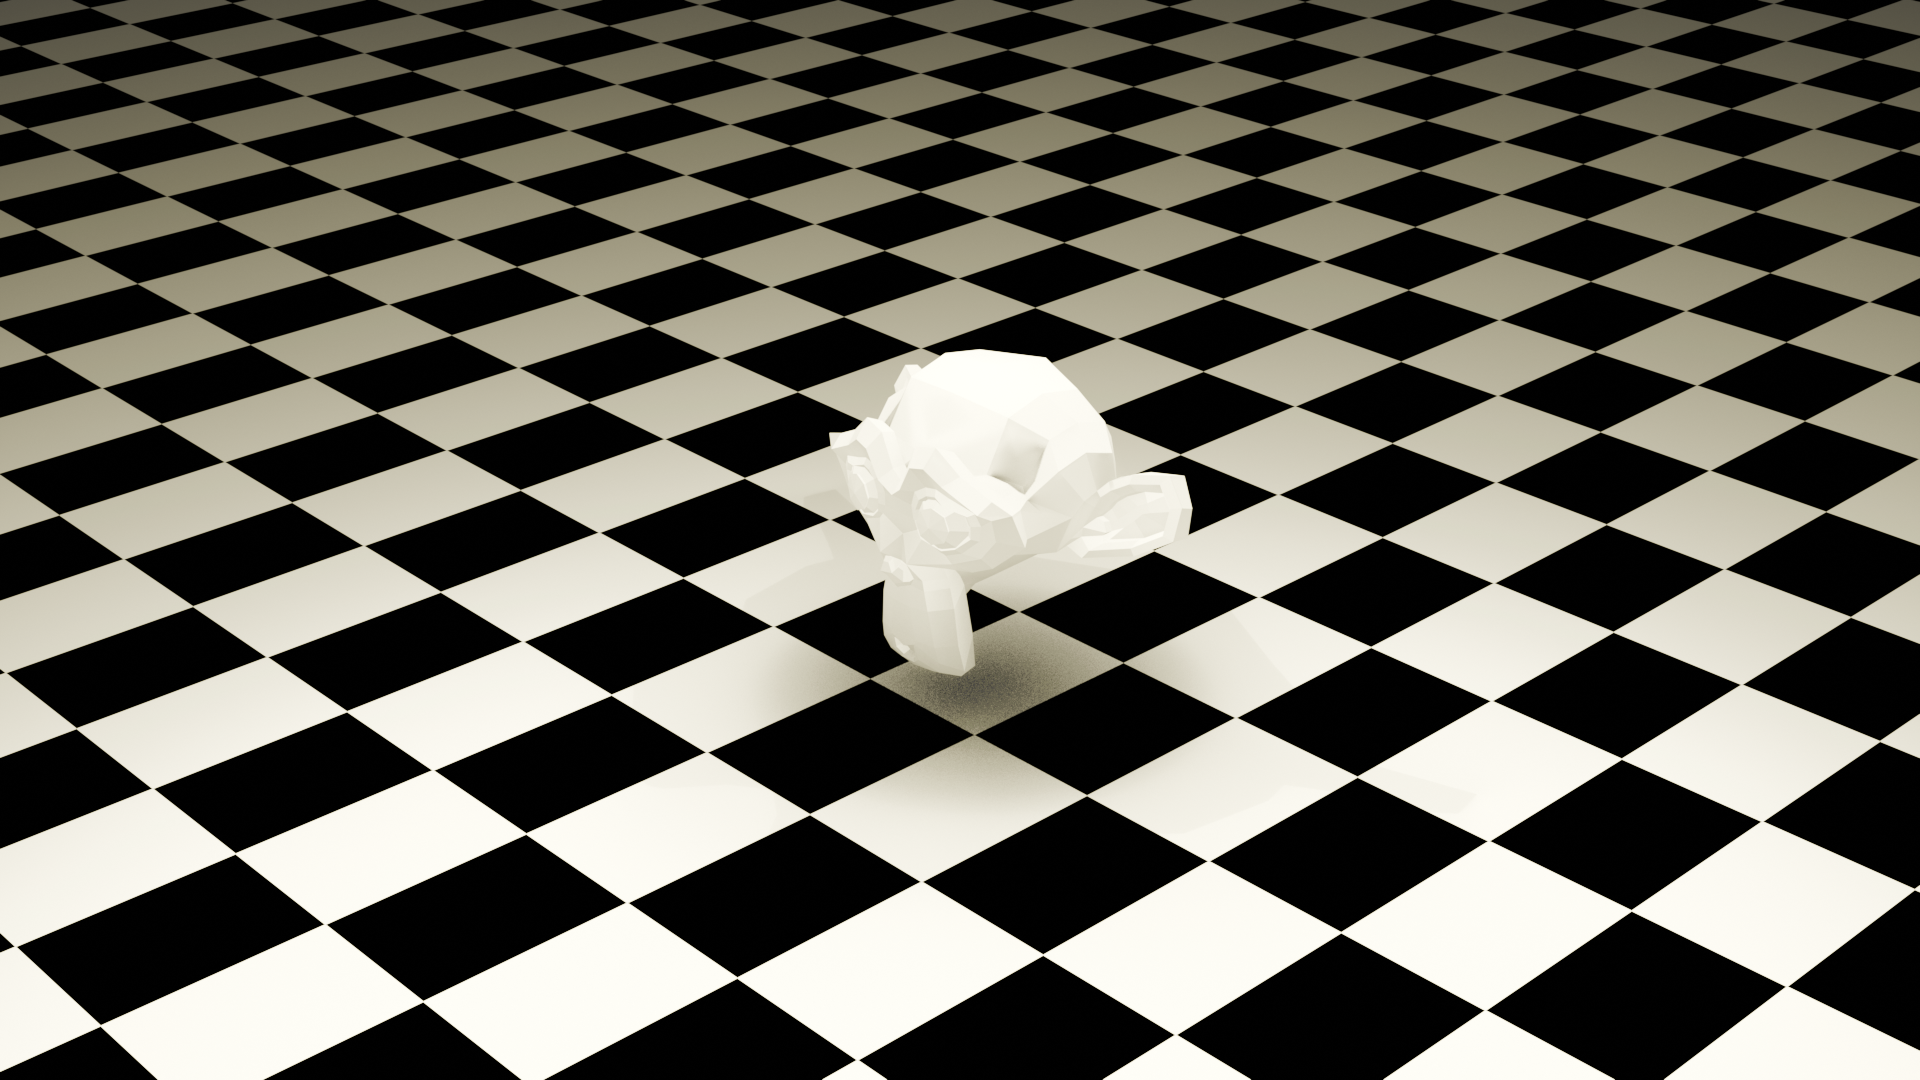
\includegraphics[width=\textwidth]{images/point_no_falloff.png}
      \caption*{No Attenuation}
    \end{minipage}
    \hfill
    \begin{minipage}{0.48\textwidth}
      \centering
      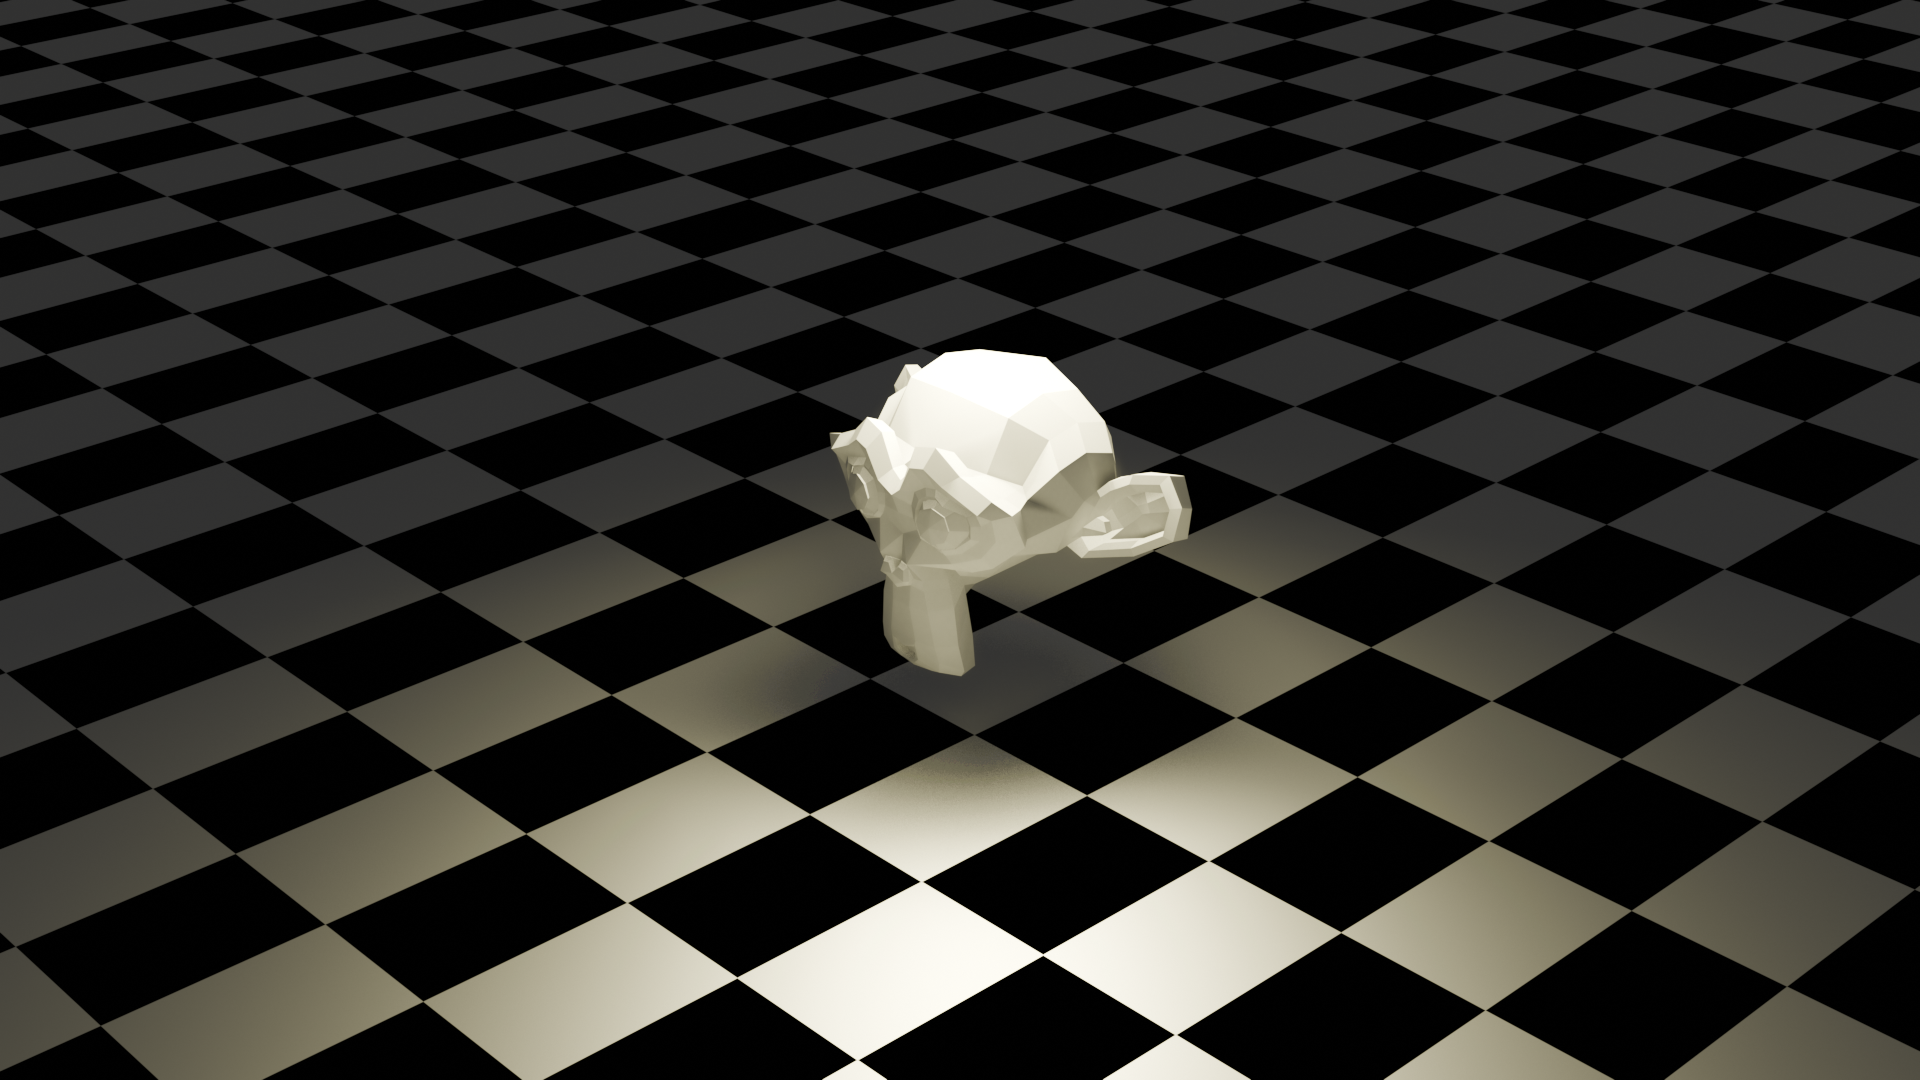
\includegraphics[width=\textwidth]{images/point.png}
      \caption*{With Attenuation}
    \end{minipage}
  \end{figure}

\end{frame}

\begin{frame}{Inverse Square Law - The Physics}
  \begin{columns}
    \begin{column}{0.6\textwidth}
      \begin{conceptbox}{$1/r^2$ Attenuation}
        \small
        \begin{itemize}
          \item \textbf{Physical principle:} Light energy spreads over larger area as distance increases.
          \item<2-> \textbf{Sphere surface area:} $A = 4\pi r^2$
          \item<3-> \textbf{Energy conservation:} Same total energy spread over larger area.
          \item<4-> \textbf{Intensity per unit area:} $I \propto \frac{1}{r^2}$
        \end{itemize}
      \end{conceptbox}

    \end{column}
    \begin{column}{0.4\textwidth}
      \begin{tikzpicture}[scale=0.6]
        % Point light
        \node[circle, fill=LightColor, minimum size=0.8cm] (light) at (0,0) {\faIcon{lightbulb}};

        % Spherical shells at different distances
        \draw[AccentColor, thick] (0,0) circle (1.5);
        \draw[AccentColor, thick] (0,0) circle (3);

        % Radius labels
        \draw[<->, thin] (0,0) -- (1.5,0) node[midway, above, xshift=0.1cm] {\footnotesize $r$};
        \draw[<->, thin] (0,0) -- (3,0) node[midway, below, xshift=0.5cm] {\footnotesize $2r$};

        % Area annotations
        \node[AccentColor] at (1.1,1.5) {\footnotesize $A_1$};
        \node[AccentColor] at (2.1,3) {\footnotesize $A_2 = 4A_1$};

        % Energy density
        \node[below] at (0,-3.5) {
          \scriptsize
          Same energy → 4× area → $\frac{1}{4}$ intensity
        };
      \end{tikzpicture}
    \end{column}
  \end{columns}

  \vspace{0.3cm}
  \only<5->{
    \begin{mathbox}{Attenuation Formula}
      \vspace*{-0.5cm}
      \begin{align*}
        I_{\text{received}} = \frac{I_{\text{light}}}{d^2} \quad \text{where } d = \text{distance to light}
      \end{align*}
    \end{mathbox}
  }
\end{frame}

\begin{frame}{Point Light Implementation}
  \begin{mathbox}{Point Light Function Structure}
    \small
    \only<1>{

      \textbf{Input parameters:}
      \begin{itemize}
        \item Light position: $\mathbf{P}_{\text{light}}$
        \item Light intensity: $I_{\text{light}}$
        \item Light color: $\mathbf{C}_{\text{light}} = (r, g, b)$
        \item Surface point: $\mathbf{P}_{\text{surface}}$
      \end{itemize}
    }
    \only<2>{

      \textbf{Calculation steps:}
      \begin{align*}
        \mathbf{L} &= \mathbf{P}_{\text{light}} - \mathbf{P}_{\text{surface}} \\
        d &= |\mathbf{L}| \\
        \hat{\mathbf{L}} &= \mathbf{L} / d \\
        I_{\text{final}} &= \frac{I_{\text{light}}}{\epsilon + d^2}
      \end{align*}
    }
  \end{mathbox}
\end{frame}
\subsection{Directional Lights}

\begin{frame}{Directional Lights - The Sun Model}
  \begin{columns}
    \begin{column}{0.6\textwidth}
      \begin{raybox}{Directional Light Concept}
        \small
        Light source at infinite distance, so rays are effectively parallel

        \only<2>{
          \vspace{0.3cm}
          \textbf{Characteristics:}
          \begin{itemize}
            \item Parallel rays
            \item Same intensity everywhere
            \item No attenuation
            \item Defined by direction only
          \end{itemize}
        }

        \only<3->{
          \vspace{0.3cm}
          \textbf{Perfect for:} Sun, moon, distant lights
        }
      \end{raybox}

      \only<4->{
        \begin{center}
          \begin{figure}
            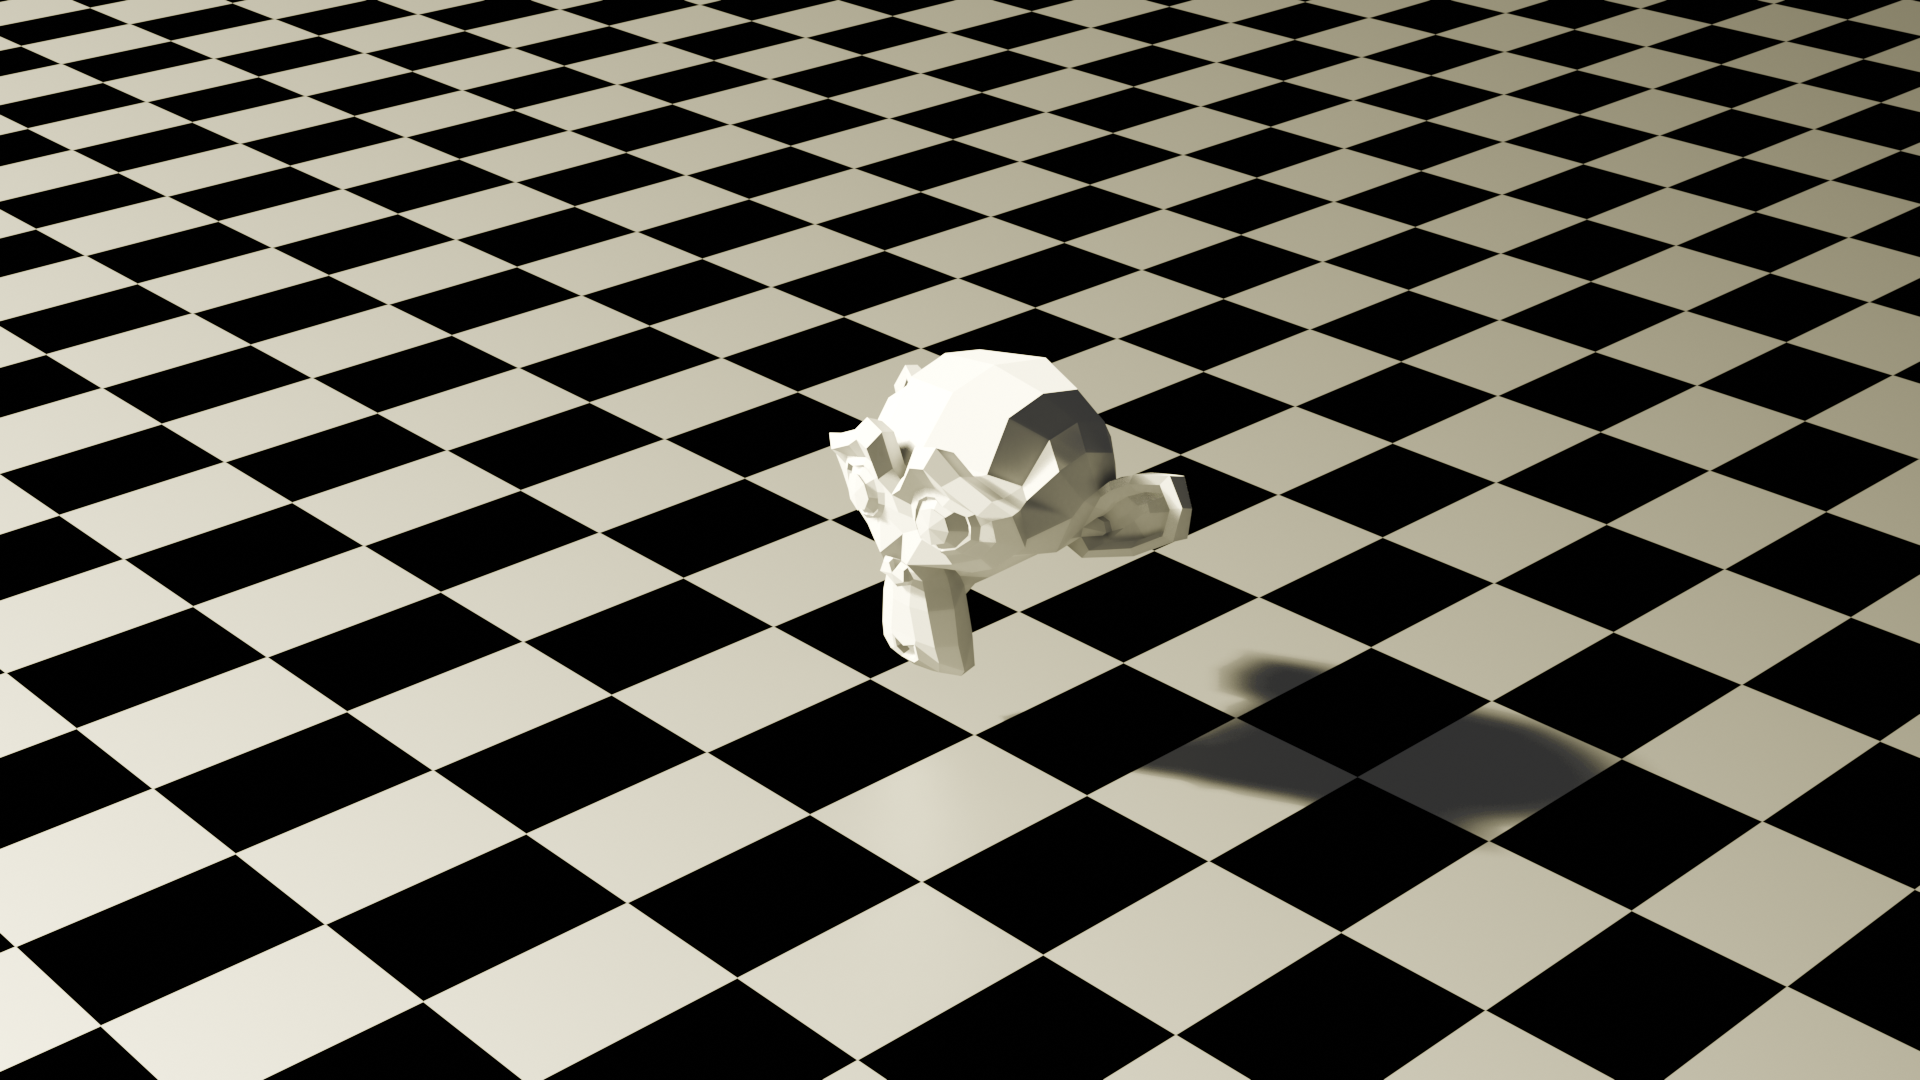
\includegraphics[width=\linewidth]{images/dir.png}
            \caption*{Directional Light ft. Suzanne}
          \end{figure}
        \end{center}
      }
    \end{column}
    \begin{column}{0.4\textwidth}
      \centering
      \scriptsize
      \begin{tikzpicture}[scale=0.5]
        % Sun (very far away)
        \node[circle, fill=LightColor, minimum size=1cm] (sun) at (-3,2) {\faIcon{sun}};
        \node[above] at (-3,2.7) {\footnotesize Sun (very far)};

        % Parallel rays
        \foreach \y in {0.5,1,1.5,2,2.5,3,3.5} {
          \draw[lightray, ->, thick] (-1,\y) -- (3.5,\y);
        }

        % Objects receiving parallel light
        \node[sphere, minimum size=0.8cm] (obj1) at (1,1) {};
        \node[sphere, minimum size=0.8cm] (obj2) at (3,3.5) {};

        % Direction vector
        \draw[->, red, very thick] (0,-2) -- (1.5,-2);
        \node[below] at (0.75,-2.3) {\footnotesize $\mathbf{L}$ (same for all points)};

        % Equal intensity indication
        \node[below] at (1,0.3) {\footnotesize Same intensity};
        \node[below] at (3,5) {\footnotesize Same intensity};
      \end{tikzpicture}
    \end{column}
  \end{columns}

\end{frame}

\begin{frame}{Directional Light Mathematics}
  \begin{columns}
    \begin{column}{0.6\textwidth}
      \begin{mathbox}{Directional Light Parameters}
        \textbf{Direction:} $\mathbf{D}_{\text{light}} = (x, y, z)$

        \textbf{Intensity:} $I_{\text{light}}$ (constant)

        \textbf{Color:} $\mathbf{C}_{\text{light}} = (r, g, b)$

        \vspace{0.3cm}
        \only<2->{
          \textbf{Light direction:}
          \begin{align*}
            \hat{\mathbf{L}} = -\mathbf{D}_{\text{light}}
          \end{align*}
          \only<2>{
            \footnotesize
            \textbf{Note:} Assuming $\mathbf{D}_{\text{light}}$ is normalized
          }
        }

        \only<3->{
          \textbf{Intensity at any point:}
          \begin{align*}
            I_{\text{final}} = I_{\text{light}} \quad \text{(no attenuation)}
          \end{align*}
        }
      \end{mathbox}
    \end{column}
    \begin{column}{0.4\textwidth}
      \begin{tikzpicture}[scale=0.8]
        \begin{scope}[plane origin={(2,1,0)},
            plane x={(1.293,1.707,0)},
            plane y={(2,1,1)},
          canvas is plane]
          \draw[ObjectColor, fill=ObjectColor!20, opacity=0.6] (0,0) circle (2);
        \end{scope}

        \node[circle, fill=LightColor, minimum size=1cm] (sun) at (2,6) {\faIcon{sun}};

        \foreach \x in {0.5,1,1.5,2,2.5,3,3.5} {
          \draw[lightray, ->, thick] (\x, 5) -- (\x,4);
        }

        % Direction vector from light
        \draw[->, lightray, very thick] (2,3) -- (2,1);
        \node[right] at (2.2,2) {\footnotesize  $\hat{\mathbf{L}} = -\mathbf{D}_{\text{light}}$};
        \node[above] at (2,3.3) {\footnotesize Light direction $\mathbf{D}_{\text{light}}$};

        % Surface point
        \fill[ObjectColor] (2,1) circle (3pt);
        \node[below] at (2,0.7) {\footnotesize Surface point};
        \draw[->, very thick, red] (2,1) -- (2,3);

      \end{tikzpicture}
    \end{column}
  \end{columns}
\end{frame}
\subsection{Spot Lights}

\begin{frame}{Spot Lights - Introduction}
  \begin{columns}
    \begin{column}{0.7\textwidth}
      \begin{raybox}{Spot Light Characteristics}
        Light emanating from a point within a cone

        \only<2>{
          \vspace{0.1cm}
          \textbf{Real-world examples:}
          \begin{itemize}
            \item Flashlights, headlights
            \item Stage spotlights
            \item Desk lamps
          \end{itemize}
        }
      \end{raybox}

      \only<3>{
        \begin{center}
          \begin{figure}
            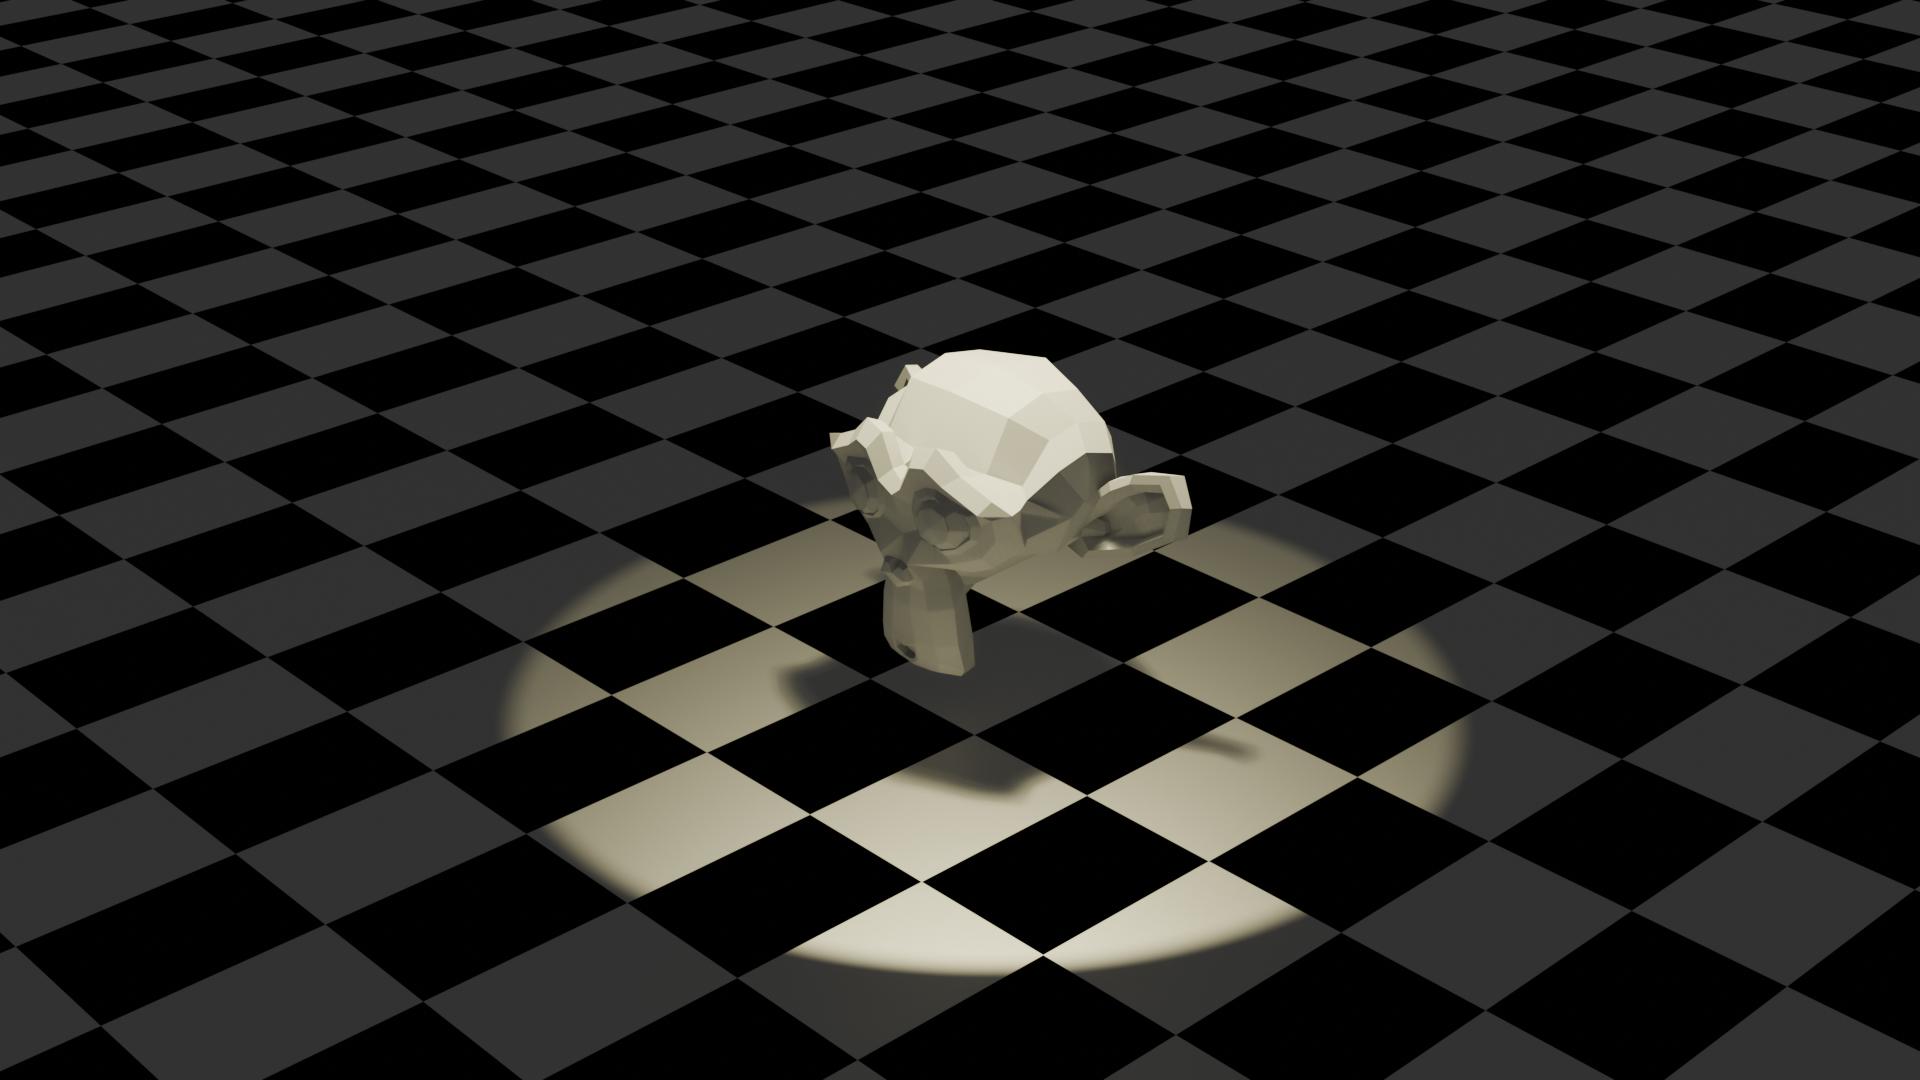
\includegraphics[width=\linewidth]{images/spot.png}
            \caption*{Spot Light ft. Suzanne the monkey}
          \end{figure}
        \end{center}
      }
    \end{column}
    \begin{column}{0.3\textwidth}
      \centering
      \begin{tikzpicture}[scale=0.8]
        \node[circle, fill=LightColor, minimum size=0.6cm] (light) at (1,3) {\footnotesize S};
        \node[above] at (1,3.5) {\footnotesize Spotlight};

        \draw[lightray, thick] (light) -- (0,0);
        \draw[lightray, thick] (light) -- (2,0);
        \draw[lightray, fill=LightColor, opacity=0.2] (light.center) -- (0,0) -- (2,0) -- cycle;

        \draw[->, red, very thick] (light) -- (1,1.5);
        \node[right] at (1.2,2.2) {\footnotesize Direction};

        \draw[-] (1, 1.25) arc [start angle=-90, end angle=-71, radius=1.75] node[midway, below] {\footnotesize $\theta$};

        \draw[dashed] (light) -- (1,0);

        \node[sphere, minimum size=0.6cm] (obj1) at (0.7,-0.5) {};
        \node[sphere, minimum size=0.6cm,fill=ObjectColor!60] (obj2) at (3,-0.5) {};

        \node[below] at (0.7,-1) {\footnotesize Lit};
        \node[below] at (3,-1) {\footnotesize Dark};
      \end{tikzpicture}
    \end{column}
  \end{columns}
\end{frame}

\begin{frame}{Spot Light Mathematics - Cone Calculation}
  \begin{columns}
    \begin{column}{0.7\textwidth}
      \begin{mathbox}{Spot Light Parameters}
        \textbf{Position:} $\mathbf{P}_l$

        \textbf{Intensity:} $\mathbf{I}_l$

        \textbf{Direction:} $\mathbf{D}_{\text{spot}}$

        \textbf{Cone angle:} $\theta_{\text{cutoff}}$

        \textbf{Falloff exponent:} $e$

        \vspace{0.3cm}
        \pause
        \textbf{Step 1 - Calculate angle to surface:}
        \begin{align*}
          \hat{\mathbf{L}} &= \frac{\mathbf{P}_l - \mathbf{P}_{\text{surface}}}
          {|\mathbf{P}_l - \mathbf{P}_{\text{surface}}|} \\
          \cos(\alpha) &=  \mathbf{D}_{\text{spot}} \cdot (- \hat{\mathbf{L}})
        \end{align*}

        \pause
        \textbf{Step 2 - Check if inside cone:}
        \begin{align*}
          \text{if } \cos(\alpha) > \cos(\theta_{\text{cutoff}}) \text{ then illuminate}
        \end{align*}
      \end{mathbox}
    \end{column}
    \begin{column}{0.3\textwidth}
      \begin{tikzpicture}[scale=0.8]
        \node[circle, fill=LightColor, minimum size=0.6cm] (light) at (3,3) {\footnotesize S};

        \begin{scope}[plane origin={(1,1,0)},
            plane x={(0.293,1.707,0)},
            plane y={(1,1,1)},
          canvas is plane]
          \draw[ObjectColor, fill=ObjectColor!20, opacity=0.6] (0,0) circle (1);
        \end{scope}

        \coordinate (surface) at (1,1);
        \fill[ObjectColor] (1,1) circle (2pt);
        \node[below] at (1,1) {\footnotesize $\mathbf{P}_{\text{surface}}$};

        \begin{scope}[shift={(3,3)}]

          \draw[->, blue, thick] (light) -- ($(light)+0.5*(surface)-0.5*(light)$) node[midway, above, anchor=south, black, xshift=-0.1cm] {\footnotesize $-\hat{\mathbf{L}}$};

          \draw[dashed] (light) -- (surface);
          \draw[dashed] (light) -- (-90:5);

          \draw[-] (0,-1) arc [start angle=-90, end angle=-135, radius=1] node[midway, below] {\footnotesize $\alpha$};
          \draw[-] (0,-2.5) arc [start angle=-90, end angle=-110, radius=2.5] node[midway, below] {\footnotesize $\theta_{\text{cutoff}}$};

          \draw[lightray, dashed] (light) -- (-70:4);
          \draw[lightray, dashed] (light) -- (-110:4);

          \draw[->, red, very thick] (light) -- (0,-2) node[midway, right, anchor=west, black] {\footnotesize $\mathbf{D}_{\text{spot}}$};
        \end{scope}

      \end{tikzpicture}
    \end{column}
  \end{columns}
\end{frame}

\begin{frame}{Spot Light Attenuation}
  \begin{mathbox}{Complete Spot Light Formula}
    \small
    \textbf{Angular attenuation:}
    \begin{align*}
      \text{spot\_factor} =
      \begin{cases}
        (\cos(\alpha))^e & \text{if } \cos(\alpha) > \cos(\theta_{\text{cutoff}}) \\
        0 & \text{otherwise}
      \end{cases}
    \end{align*}
    \only<2>{
      The $e$ exponent controls how much brighter the light is at the center of the cone compared to the edges.
    }

    \only<3->{
      \textbf{Distance attenuation} (same as point light):
      \begin{align*}
        \text{distance\_attenuation} = \frac{1}{\epsilon + d^2}
      \end{align*}
    }

    \only<4->{
      \textbf{Final intensity:}
      \begin{align*}
        I_{\text{final}} =
        \begin{cases}
          \mathbf{I}_l \cdot (\cos(\alpha))^e \cdot \frac{1}{\epsilon + d^2} & \text{if } \cos(\alpha) > \cos(\theta_{\text{cutoff}}) \\
          0 & \text{otherwise}
        \end{cases}
      \end{align*}
    }
  \end{mathbox}
  \only<2>{
    \begin{figure}
      \centering
      \begin{columns}
        \begin{column}{0.25\textwidth}
          
\includegraphics[width=\linewidth]{images/spot_e_0.png}
          \centering
          {\footnotesize $e=0$}
        \end{column}
        \begin{column}{0.25\textwidth}
          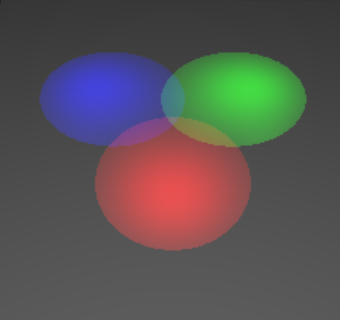
\includegraphics[width=\linewidth]{images/spot_e_10.png}
          \centering
          {\footnotesize $e=10$}
        \end{column}
        \begin{column}{0.25\textwidth}
          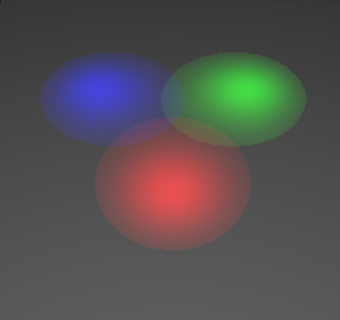
\includegraphics[width=\linewidth]{images/spot_e_20.png}
          \centering
          {\footnotesize $e=20$}
        \end{column}
        \begin{column}{0.25\textwidth}
          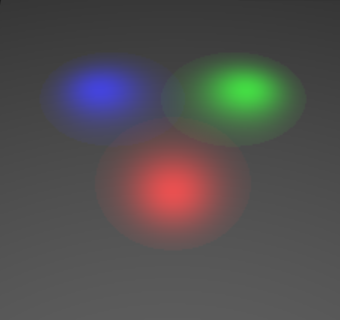
\includegraphics[width=\linewidth]{images/spot_e_30.png}
          \centering
          {\footnotesize $e=30$}
        \end{column}
      \end{columns}
      \caption*{Spot lights for different values of $e$}
    \end{figure}
  }
\end{frame}

\subsection{Ambient Light}

\begin{frame}{Ambient Light - Global Illumination Approximation}
  \begin{columns}
    \begin{column}{0.6\textwidth}
      \only<1-2>{
        \begin{conceptbox}{Direct Lighting Problem}
          \small
          Real scenes have indirect lighting
          \begin{itemize}
            \item Light bounces off walls, ceiling
            \item Reflections illuminate shadows
            \item Even "dark" areas receive some light
          \end{itemize}
        \end{conceptbox}
      }

      \only<3>{
        \begin{raybox}{Solution: Ambient Light}
          \small
          Add constant ambient term
          \begin{itemize}
            \item Prevents completely black shadows
            \item Approximates global illumination
            \item Simple and fast to compute
          \end{itemize}
        \end{raybox}
      }
      \only<4->{
        \begin{conceptbox}{Ambient Light Parameters}
          \textbf{Ambient intensity:} $I_{\text{light}}$ (constant)

          \textbf{Color:} $\mathbf{C}_{\text{light}} = (r, g, b)$
        \end{conceptbox}
      }
    \end{column}
    \begin{column}{0.4\textwidth}
      \only<1>{
        \begin{tikzpicture}[scale=0.8]
          \draw[thick] (0,0) -- (3,0) -- (3,3) -- (0,3) -- cycle;
          \node[circle, fill=LightColor, minimum size=0.6cm] (light) at (1.5,2.5) {};

          \draw[lightray] (light) -- (3,1.5);
          \draw[lightray] (light) -- (0,1.25);

          \draw[lightray, dashed, opacity=0.6] (3,1.5) -- (2,0);
          \draw[lightray, dashed, opacity=0.6] (2,0) -- (1,0.5);
          \draw[lightray, dashed, opacity=0.6] (0,1.25) -- (0.5,0);
          \draw[lightray, dashed, opacity=0.6] (1,0.5) -- (0.75,0);

          \node[sphere, minimum size=0.6cm] (obj) at (1,1) {};

          \node[right] at (3.2,2) {\footnotesize Direct light};
          \node[right] at (3.2,1) {\footnotesize Bounced light};

          \node[below] at (0.625, 0) {\footnotesize Indirect light};
        \end{tikzpicture}
      }
      \only<2->{
        \begin{figure}
          \centering
          \only<2>{
            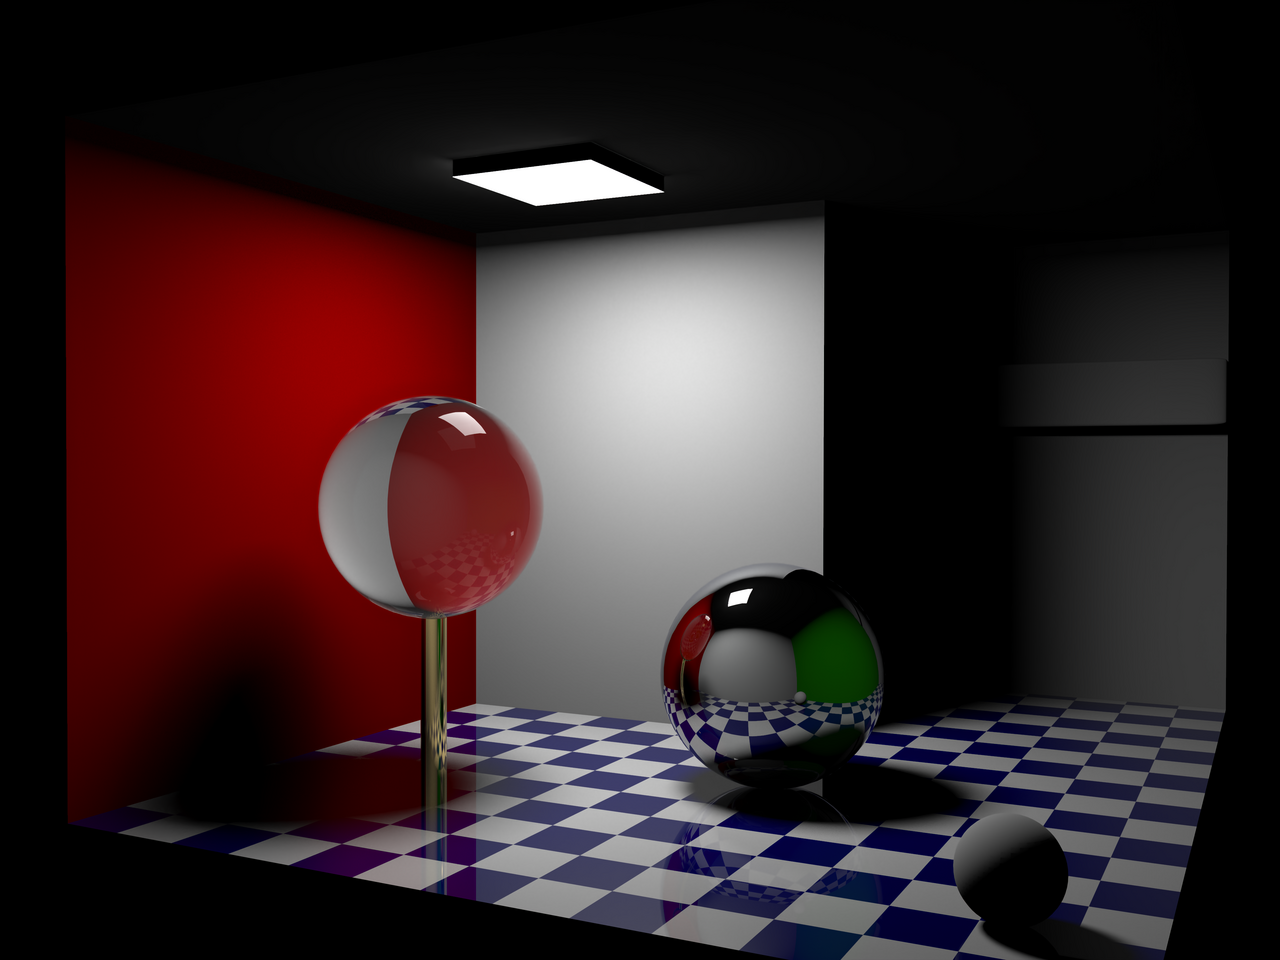
\includegraphics[width=0.8\textwidth]{images/no_gi.png}
            \caption*{Only direct light}
            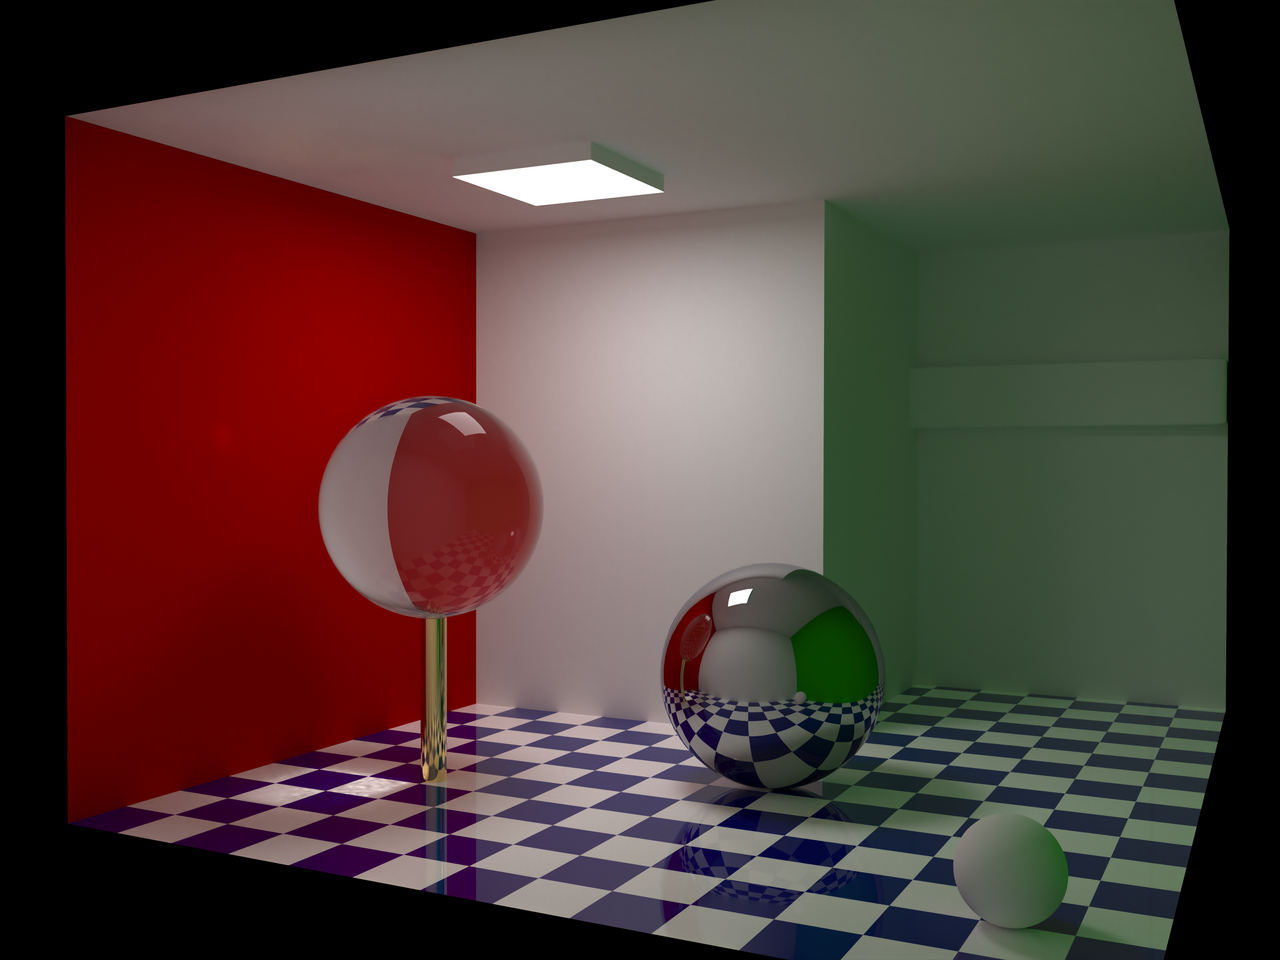
\includegraphics[width=0.8\textwidth]{images/gi.png}
            \caption*{Global illumination}
          }
          \only<3->{
            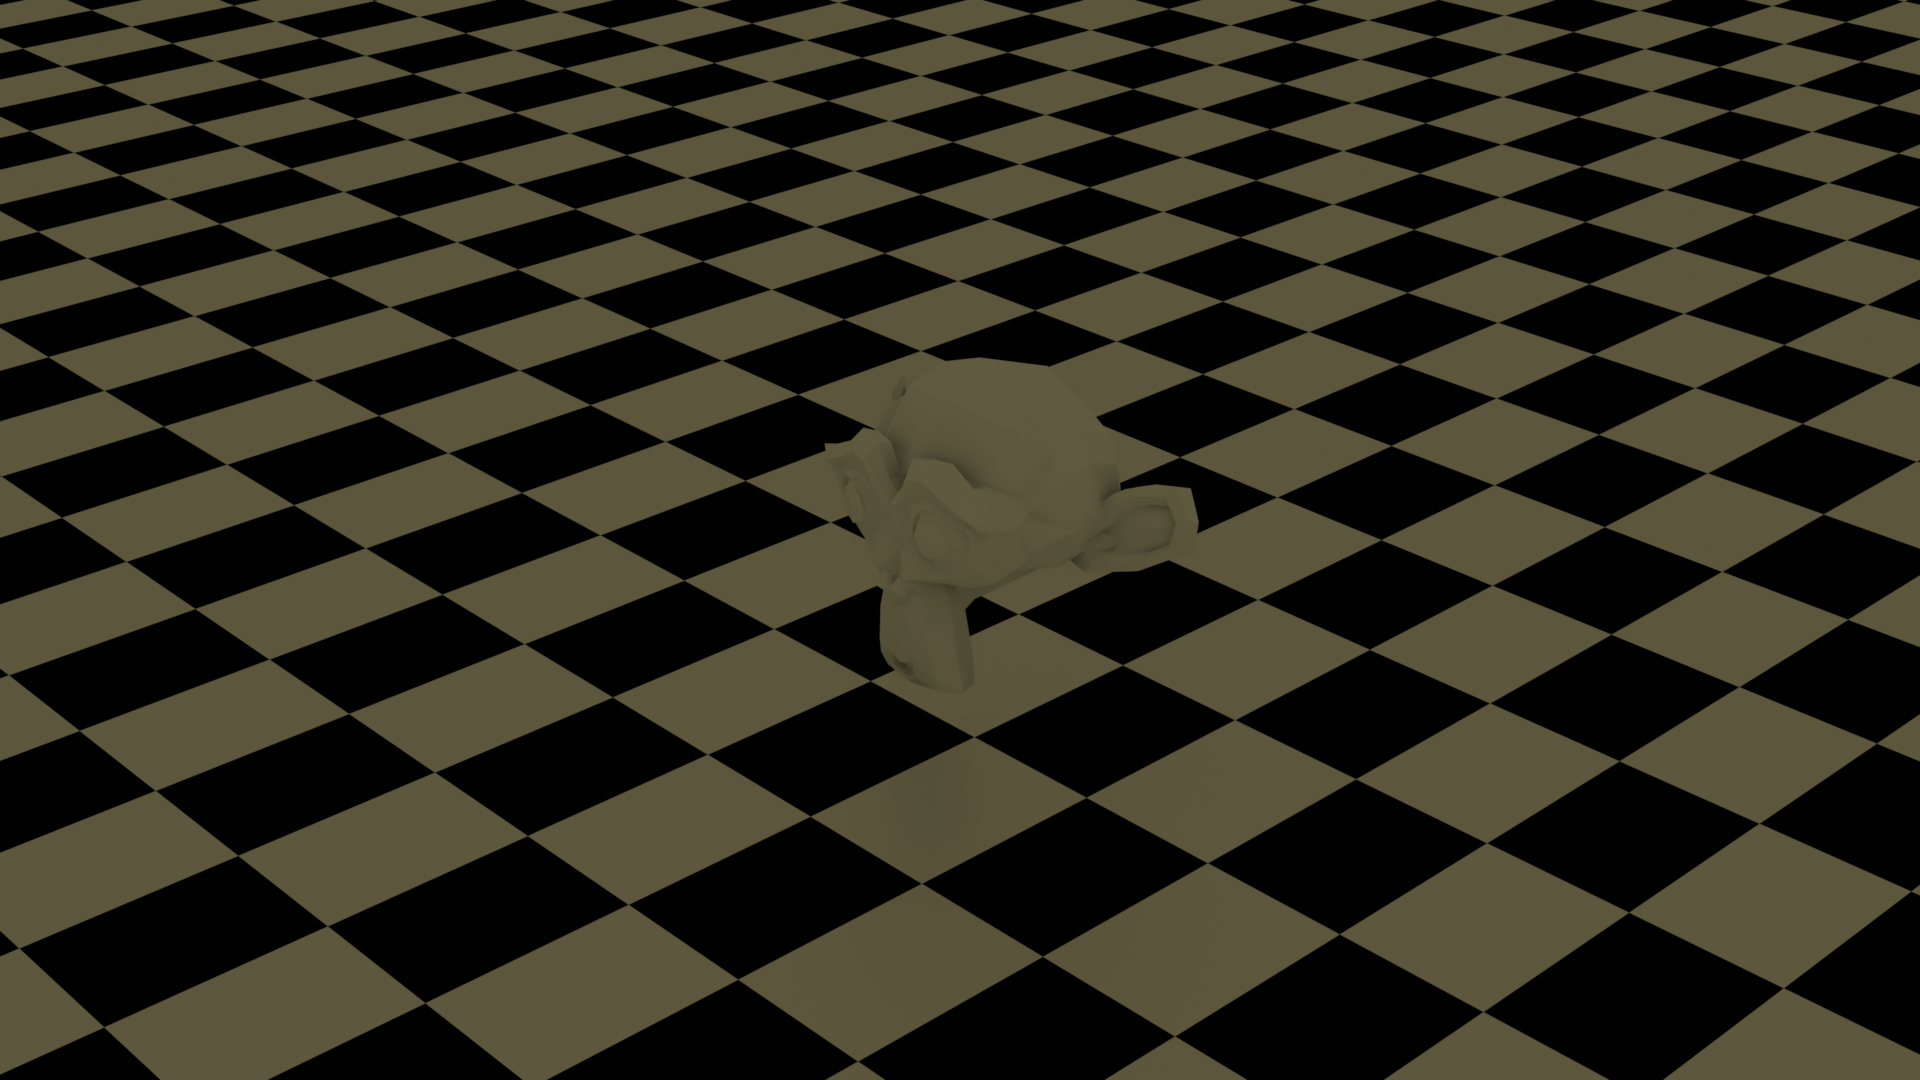
\includegraphics[width=0.8\textwidth]{images/ambient.png}
            \caption*{Ambient light ft. Suzanne the monkey}
          }
        \end{figure}
      }
    \end{column}
  \end{columns}
\end{frame}
